\chapter{绪论}
\label{chap:intro}
% ============================================================
\section{研究背景与意义}
% ============================================================

天地一体化信息网络是支撑未来全球通信、遥感感知、任务协同与智能服务的重要基础设施，也是推动空天信息系统由传统“数据传输网络”向“综合信息处理网络”演进的关键方向。随着低轨卫星星座持续部署、星间链路逐步完善以及星载计算平台能力不断提升，卫星节点的功能定位正在发生深刻变化。传统卫星网络更多承担透明转发与数据中继功能，而新一代天基网络则逐步具备在轨处理、任务协同、资源调度和自治管控等能力，正在由单纯的信息传输载体演进为面向复杂业务场景的分布式协同计算平台。对于天地一体化信息网络而言，这种演进不仅意味着网络服务能力的提升，也意味着网络运行模式、任务组织方式与资源管理机制的系统性变革\cite{ref1,ref2,ref3}。

从现实应用需求看，天基网络正在承担越来越多高时敏、高动态和高自治要求的业务任务。在灾害应急通信、对地观测快速处理、区域目标识别、空间态势感知、海洋与航运监测以及跨区域任务协同等场景中，系统不仅需要完成数据采集和远程传输，还需要在有限可见窗口、受限链路条件和复杂任务环境下实现任务接入、资源协调、计算处理与结果反馈的快速闭环。尤其是在突发灾害、局部冲突、复杂海域巡检等场景中，任务往往具有突发性、密集性和强时效性，若仍然依赖传统“星上初步处理—地面集中分析”的工作模式，则容易受到星地链路时延、可见窗口受限以及地面中心计算负载瓶颈等因素制约，难以满足高时敏业务对于快速响应和在轨闭环处理的实际需求\cite{ref2,ref4}。

在此背景下，将计算能力由地面向星上前移，并在多颗卫星之间实现资源共享与协同处理，已成为提升天基网络智能服务能力的重要发展方向。与仅依赖地面中心的集中处理模式相比，星上计算能够缩短数据处理链路、降低回传压力、提升任务响应速度；而进一步引入多星协同计算，则有望突破单颗卫星在算力、能量、存储和链路条件等方面的资源限制，在更大空间范围内实现任务迁移、负载分担和算力共享，从而增强天基网络在复杂动态场景下的综合服务能力。

图~\ref{fig:scenario}给出了天基网络协同计算卸载的典型应用场景。在该场景中，地面突发任务首先通过上行链路接入过载卫星，过载卫星在本地资源不足或任务积压严重时，可将部分任务经由星间链路卸载至资源相对空闲的卫星节点执行；同时，区块链/多智能体管控层对各卫星节点的资源状态、协同关系和策略执行过程进行支撑，实现状态共享、共识记账与策略协同，最终将处理结果回传地面。该图较为直观地反映了本文所关注问题的典型特征，即高动态环境下多节点之间的任务迁移、资源协调、可信共享与协同决策问题。

\begin{figure}[htbp]
  \centering
  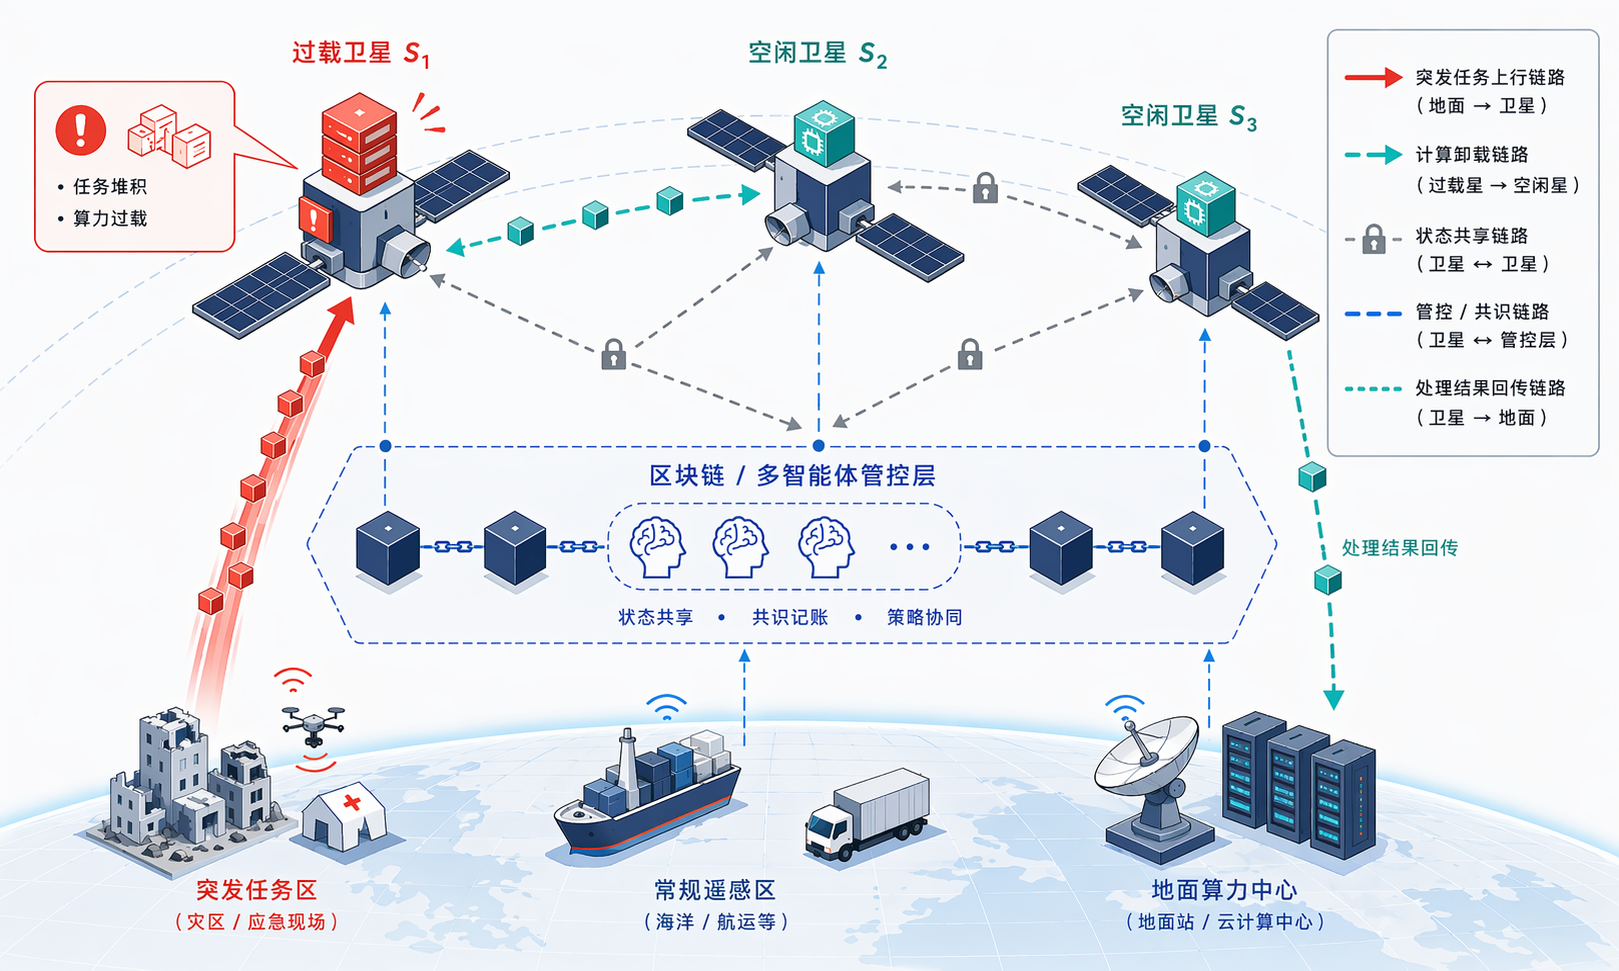
\includegraphics[width=0.85\textwidth]{figures/1-1.png}
  \caption{天基网络协同计算卸载应用场景}
  \label{fig:scenario}
\end{figure}

从现有技术体系看，面向天基网络任务处理需求，当前计算能力部署方式主要可归纳为星地集中处理、星上本地处理、星间协同处理以及分布式智能管控等几种典型模式。不同模式在支撑基础、服务能力和适用范围等方面各有特点，但同时也存在明显局限。为更清晰地说明不同模式的适用性与不足，表~\ref{tab:computing_modes}给出了典型天基网络计算模式及其技术特点对比。

\begin{table}[htbp]
  \centering
  \caption{典型天基网络计算模式及其技术特点}
  \label{tab:computing_modes}
  \begin{tabularx}{\textwidth}{CCCC}
    \toprule
    \textbf{计算模式} & \textbf{核心支撑}   & \textbf{主要能力}    & \textbf{典型局限}         \\
    \midrule
    星地集中处理        & 地面中心、馈电链路       & 适合离线分析与统一调度      & 受星地时延、可见窗口和回传带宽限制     \\
    星上本地处理        & 星载处理器、单星资源      & 支持任务就地预处理与快速响应   & 受单星算力、功耗与能量循环约束       \\
    星间协同处理        & 星间链路、多星协同       & 支持跨节点算力共享与任务迁移   & 动态拓扑下状态获取与决策复杂        \\
    分布式智能管控       & 区块链、MARL、FL、DRL & 支持可信共享、协同博弈与智能卸载 & 需同时解决共识开销、协同稳定与代价预测问题 \\
    \bottomrule
  \end{tabularx}
\end{table}

如表~\ref{tab:computing_modes}所示，星地集中处理模式依托地面中心强大的存储和计算资源，适合完成统一分析、全局调度与离线决策，但其运行效果高度依赖星地链路质量、卫星可见窗口和回传带宽条件，当任务具有强实时性要求时，该模式的闭环响应能力往往受到限制。相比之下，星上本地处理模式能够在数据产生位置附近完成预处理与快速决策，具有较好的实时性优势，但单颗卫星受平台尺寸、载荷能力、功耗预算、热控条件以及轨道能量循环等因素约束，难以长期承担高强度、连续化、多任务并发的计算需求。当任务密集到达或局部区域业务突发增长时，单节点容易出现排队积压、执行时延抬升以及任务失效等问题。

正是在上述矛盾推动下，星间协同处理逐渐成为天基网络计算能力提升的重要路径。所谓协同计算卸载，是指当任务接入卫星本地资源不足或本地执行代价过高时，通过星间链路将任务迁移至其他具备可用资源的协同节点执行，从而在更大范围内实现算力共享与负载分担\cite{ref1,ref5}。与传统纯星地集中处理模式相比，协同计算卸载能够更灵活地利用多节点资源；与单星本地处理模式相比，其能够突破单节点资源上限，在降低任务时延、提高系统吞吐量和增强网络鲁棒性方面具有明显优势。因此，协同计算卸载已成为天基网络由“可通信”向“可协同、可计算、可自治”演进过程中的关键技术之一。

然而，天基网络中的协同计算卸载并不是传统意义上的简单任务迁移问题。与地面云计算、边缘计算环境相比，天基网络中的节点资源更加受限、链路拓扑变化更加频繁、运行环境更加动态复杂。卫星高速运动使得网络拓扑、链路质量、覆盖关系和可见窗口持续变化，不同卫星节点在剩余算力、存储资源、链路状态和能量水平等方面往往存在显著异质性。与此同时，多颗卫星在同一时刻既可能是任务发起方，也可能是资源提供方，节点之间普遍存在资源竞争、收益耦合和协同行为。由此决定了天基协同计算卸载不仅要解决“任务是否卸载、卸载到哪里”的问题，更要解决高动态、去中心化环境下多节点之间的状态共享、协同博弈、实时决策与执行保障问题。

进一步而言，天基协同计算卸载的复杂性主要体现在以下几个层面。

首先，在信息层面，需要解决高动态环境下的可信状态共享问题。无论是节点间的资源协调，还是单任务的卸载决策，都依赖于对节点算力占用、剩余能量、链路连通性、队列长度和任务排队状态等信息的及时获取。然而在天基网络中，若仅依赖频繁广播实现全局状态同步，不仅会带来较大的通信开销，还可能由于链路时延、局部信息失真和同步滞后导致认知不一致。更重要的是，在去中心化的天基环境中缺乏长期稳定且可信的中心控制节点，一旦共享状态出现滞后、篡改或偏差，后续资源调度与任务卸载就可能失去可靠依据。因此，如何为多节点协同决策提供可追溯、可信任、低冲突的状态共享基础，是实现协同计算卸载的首要前提。

其次，在决策层面，需要同时面对系统层协同和任务层执行两类问题。一方面，在多颗卫星同时发起卸载请求的场景下，优质节点极易成为竞争焦点。若各节点仅从局部收益出发进行贪婪选择，则容易引发策略震荡、热点聚集、负载失衡和资源抢占等问题，影响系统整体运行效率。另一方面，任务进入目标节点后并非立即进入理想执行状态，而是会受到排队延迟、上下文切换、缓存竞争、内存争用以及功耗波动等多种并发因素影响。由此，任务层卸载决策不仅要考虑传输时延与计算时间，还需要进一步考虑更贴近真实运行环境的执行代价，才能保证卸载策略在高负载和复杂动态场景下仍具备实际有效性。

再次，在实现层面，需要解决算法方法与系统平台之间的统一承载问题。对于天基协同计算卸载而言，仅有卸载模型或优化算法并不足以支撑系统的长期稳定运行。系统层协同方法需要状态同步、规则执行、行为记录和可信审计机制作为支撑；任务层实时决策方法则依赖模型版本管理、执行反馈、结果回流以及跨节点可追溯记录。若缺乏统一的平台承载，相关方法往往停留在算法验证或离线仿真层面，难以形成可部署、可验证、可持续演进的实际运行体系。因此，从平台视角统筹考虑可信共享、协同优化、模型治理和执行反馈，同样是天基协同计算卸载研究不可回避的重要内容。

综上可见，天基协同计算卸载并不是单一节点上的局部任务调度问题，而是涉及任务接入、状态共享、跨节点协同、资源竞争、执行扰动以及结果回传等多个环节的系统性问题。该问题既具有典型的高动态、异构、去中心化特征，又包含状态可信、协同博弈和实时决策等多层耦合关系。传统依赖静态假设或中心控制的处理思路，已难以满足复杂天基环境下多节点协同计算的实际需求。因此，有必要面向可信共享、系统层协同优化、任务层实时卸载决策以及平台化承载机制开展联合研究，构建更加适应天基网络运行特征的协同计算卸载方法体系。

基于上述背景，本文围绕天基网络协同计算卸载中的关键问题展开研究，重点关注高动态环境下的可信状态共享、多节点协同资源博弈、并发感知任务卸载以及双层智能方法的平台化承载等内容。本文认为，天基协同计算卸载研究不仅在工程应用层面对提升灾害应急、遥感快处理、空间任务协同和边远区域信息服务等能力具有重要价值，而且在理论与方法层面也可为高动态、去中心化、资源受限网络环境中的分布式协同计算研究提供新的思路。通过构建兼顾可信共享、系统协同、任务决策与平台承载的统一研究框架，有望提升天基网络在复杂任务场景下的实时响应能力、资源利用效率与智能自治水平，为天地一体化信息网络向智能化、协同化和自治化方向发展提供理论支撑与技术参考。

% ============================================================
\section{国内外研究现状与发展趋势}
% ============================================================

围绕天基网络协同计算卸载问题，国内外研究已从体系架构、任务卸载、智能调度、去中心化协同、隐私保护建模以及平台化支撑等多个角度展开探索。总体来看，相关研究正沿两个方向并行推进：一方面，卫星边缘计算与星间协同处理不断走向实用化，任务卸载与资源调度问题逐步由静态建模转向动态学习；另一方面，随着网络规模扩张和节点自治能力增强，可信共享、分布式共识、联邦学习以及区块链平台等支撑机制日益成为研究重点。基于此，本节从天基边缘计算与卸载、动态环境下的智能调度、多节点可信协同与隐私保护三个方面进行梳理，并据此明确本文的研究定位。

\subsection{天基网络与卫星边缘计算研究现状}

随着低轨卫星星座的快速发展，卫星边缘计算已成为天基网络研究中的热点方向。已有研究普遍认为，未来卫星网络不应仅承担透明转发功能，而应具备在轨预处理、局部协同分析和边缘服务承载能力，以缓解地面中心压力并提升实时响应能力\cite{ref1,ref4}。围绕这一目标，学界先后提出星地协同、星间协同和天地融合等多种计算架构，试图根据任务复杂度、时延要求和资源约束，在终端、卫星与地面之间灵活划分处理位置。

在具体卸载方法方面，早期研究多采用解析优化、启发式搜索或博弈论方法，对时延、能耗和资源利用率进行联合建模。这类方法在问题规模较小且假设条件较强时具有较好的可解释性，但当网络拓扑频繁变化、链路状态动态波动或任务到达具有突发性时，其模型有效性往往难以长期保持。例如，Gao等针对LEO星座网络中的分布式动态卸载问题，基于博弈论建立了联合计算卸载与功率分配模型，在分布式环境下优化了资源利用效率，但该方法的求解过程依赖较强的信道静态假设\cite{ref19}。

自2024年以来，相关研究开始更加重视卸载问题中的时变信道、队列状态和动态负载因素。Jia等提出面向卫星边缘计算的深度多智能体强化学习方法MATORA，将任务卸载与资源分配拆分求解，在动态负载条件下提高了时延优化能力\cite{ref3}。Li等针对LEO卫星边缘计算网络研究了基于MADDPG的联合卸载与资源分配问题，通过分布式学习处理高动态环境中的能耗与时延折中\cite{ref2}。Shuai等讨论了基于Q-learning的卫星边缘计算卸载策略，进一步验证了强化学习方法在动态卫星场景中的适应性\cite{ref5}。与此同时，Tang等研究了基于星间链路的星地一体化网络任务卸载与资源分配问题，提出混合云与卫星多层多接入边缘计算架构，通过联合优化节点选择、卸载比率和算力分配实现了网络资源的动态管理\cite{ref20}。

进入2025年以后，研究重点进一步从“是否卸载”扩展到“如何在多目标条件下稳定卸载”。Xu等提出面向卫星边缘计算的多目标强化学习卸载方法，将时延、资源利用率和负载均衡纳入统一优化目标，改善了复杂任务场景下的综合性能\cite{ref15}。Ma等则着重分析了任务优先级、资源竞争和联合分配之间的耦合关系，指出卸载研究正在由单一指标优化转向优先级感知、服务质量约束和多资源联合编排\cite{ref16}。在此基础上，Wang等提出MARATD3算法，将循环神经网络与多头注意力机制引入多智能体深度确定性策略梯度框架，在部分可观测条件下实现了跨时隙的动态卸载与资源分配联合优化，为高动态卫星环境中的序贯决策问题提供了新的建模范式\cite{ref21}。与此同时，Jia等探索了联邦深度强化学习在低轨卫星边缘计算中的应用，将联邦学习与DRL相结合，在保护用户数据隐私的同时优化计算卸载策略，指出联邦学习不仅能够保护隐私，还可作为卸载策略训练的分布式支撑手段\cite{ref22}。

这些研究表明，卫星边缘计算与任务卸载已由概念验证阶段逐步迈向细粒度建模与智能优化阶段。2024—2026年天基计算卸载与智能调度领域的代表性研究如表~\ref{tab:offloading_survey}所示。

\begin{table}[htbp]
  \centering
  \caption{2024—2026年天基计算卸载与智能调度代表研究}
  \label{tab:offloading_survey}
  \begin{tabularx}{\textwidth}{cCCC}
    \toprule
    \textbf{研究方向} & \textbf{代表文献}                & \textbf{主要内容}                       & \textbf{不足或启示}                 \\
    \midrule
    卫星边缘计算架构      & \cite{ref1,ref4}             & 从星地融合、星间协同和天地一体化角度讨论卫星边缘计算架构与业务承载方式 & 侧重体系层面描述，对协同决策机制的讨论不足          \\
    \addlinespace
    博弈论与优化方法      & \cite{ref19,ref20}           & 利用博弈论、凸优化或分层架构处理卸载与资源联合分配           & 依赖较强的信道平稳或全局信息可获得假设            \\
    \addlinespace
    单智能体RL卸载      & \cite{ref5,ref15}            & 利用Q-learning、DQN及其改进模型优化卸载时延和资源利用率  & 多从单节点或单任务视角建模，难以处理多节点博弈        \\
    \addlinespace
    MARL联合优化      & \cite{ref2,ref3,ref16,ref21} & 将多颗卫星建模为多智能体，联合优化卸载、功率、带宽和资源分配      & 通常假设状态可获得，可信共享基础偏弱             \\
    \addlinespace
    联邦学习辅助卸载      & \cite{ref22}                 & 将联邦学习与DRL结合，保护隐私同时优化卸载策略            & 联邦学习与卸载决策的闭环耦合仍待深化             \\
    \addlinespace
    2026新趋势       & \cite{ref18}                 & 引入大模型处理复杂状态下的卸载与资源分配                & 表明卸载研究向更复杂决策模型演进，但对系统层信任问题涉及较少 \\
    \bottomrule
  \end{tabularx}
\end{table}

尽管相关研究已取得显著进展，但仍存在两方面关键局限。其一，多数工作默认系统能够获得较准确的全局或准全局状态，对高动态拓扑下的状态不一致、信息失真和分布式认知偏差问题考虑不足。其二，大量模型仍将任务代价简化为传输时间与纯计算时间的线性叠加，对多任务并发带来的内部竞争和执行扰动刻画不够充分。换言之，天基计算卸载虽已从静态优化走向动态学习，但在“可信共享”和“并发感知”两个维度上仍有待深入研究。

\subsection{动态环境下智能调度与多智能体协同研究现状}

天基网络环境具有高动态、强耦合和多主体并存等特征，面向动态环境的智能调度已成为近年来相关研究的核心方向。深度强化学习之所以被广泛引入，在于其能够在缺乏精确解析模型的条件下，通过与环境持续交互形成状态到动作的映射关系，从而有效处理链路波动、任务到达随机性和资源时变性等问题\cite{ref14}。

在单智能体强化学习阶段，研究通常聚焦单节点视角下的卸载动作、功率控制或链路选择，通过DQN、DDQN、D3QN等方法提升策略对复杂状态的适应能力。此类方法在小规模、中心化或弱耦合场景中效果较好，但当多个卫星节点同时参与决策时，其隐含的“环境平稳”假设不再成立。对任一节点而言，其他节点的动作会持续改变其观测环境和收益分布，导致单智能体方法面临显著的环境非平稳性问题。

基于这一认识，多智能体强化学习在天基计算调度中日益受到重视。2024年以后，多项研究明确将多颗卫星建模为多智能体系统，通过集中训练分布执行（CTDE）或共享奖励等机制处理节点间的策略耦合关系\cite{ref2,ref3}。在CTDE范式的具体实现方面，Wu等提出了面向LEO卫星网络的多智能体深度强化学习卸载与路由联合优化方法，将计算和路由需求同时纳入多智能体建模框架，在动态负载和拓扑变化条件下展现了分布式决策的灵活性\cite{ref23}。Qin等则从可持续计算角度出发，利用MARL解决星地一体化网络中的计算卸载问题，强调全局奖励设计在多智能体收敛中的关键作用\cite{ref1}。

此类方法的核心优势在于能够同时考虑局部选择与全局负载之间的关系，使卸载策略从局部最优逐步逼近系统层协调。从当前发展趋势看，MARL在天基网络中的定位已由辅助优化工具转变为描述多节点协同演化的方法论基础。这一趋势在2025—2026年间表现得尤为明显。在卫星对地观测调度领域，AAAI 2025接收的一项工作将MARL应用于大规模序贯卫星任务分配问题，通过从多项式时间贪心求解器引导学习并结合分布式最优分配机制，成功扩展至数百个智能体和任务的规模，显著超越了先前方法\cite{ref24}。与此同时，2026年的一项研究提出时空感知的MAPPO方法，用于周期性重访约束下的多星观测调度，并通过多目标奖励函数平衡任务完成率、首次观测时效性和重访均匀度\cite{ref25}。这些工作进一步表明，MARL不仅适用于通信层面的资源分配，也正在向观测调度、联合计算与通信优化等更广泛的星上任务管控领域扩展。

需要指出的是，近年来还出现了将强化学习与联邦学习相结合的新趋势，以解决天基网络中分布式决策的隐私和通信效率问题。Han等研究了星地一体化网络中联邦学习的合作卸载问题，联合优化本地计算和数据卸载策略，为联邦学习在天基协同场景中的部署提供了理论框架\cite{ref26}。这一方向的出现，意味着智能调度正由“集中式学习后分布式部署”向“训练与部署全程分布式”演进。

与此同时，随着研究由“单一算法性能提升”走向“复杂系统长期运行优化”，越来越多工作开始关注调度算法与系统支撑环境之间的关系。换言之，多智能体协同并不只是算法选择问题，还涉及状态同步、规则执行、行为记录和跨层反馈等系统性条件。若缺乏统一的平台承载，即便算法本身能够在仿真环境中获得较好效果，也难以在真实分布式系统中持续稳定运行。这也说明，天基智能调度研究正由“算法导向”逐步迈向“算法—机制—平台”协同设计的新阶段。

然而，现有智能调度研究仍存在两个值得关注的问题。第一，许多研究虽采用多智能体框架，却仍默认节点间可以高效、真实地共享状态信息，对分布式系统中的虚假共享、状态滞后和认知不一致问题讨论不足。第二，部分工作侧重于算法收敛与指标提升，对“高动态去中心化环境为何必须采用多智能体协同而非中心化控制”的论证不够充分。实际上，MARL在天基网络中的核心价值不仅在于提升数值性能，更在于为去中心化资源博弈提供统一的建模与求解框架。

\subsection{区块链协同与隐私保护学习研究现状}

随着天基网络从封闭体系向开放协同体系演进，可信共享与去中心化协同问题日益突出。传统中心控制模式虽便于统一管理，但在大规模低轨星座和多主体参与环境下，容易面临单点失效、扩展性不足以及状态采集开销过高等问题。为此，近年来研究开始尝试引入区块链、分布式共识和自治网络协议，为天基网络构建新型协同机制。

2024年以来，该方向的代表性工作明显增多。Oh等提出去中心化多方低轨网络（MP-LEO）设想，强调通过分布式控制和多方协同共享冗余能力，提升未来卫星网络的鲁棒性与可用性\cite{ref6}。Yan等从网络协议层面提出面向通信卫星服务的去中心化协议，利用区块链式状态发布机制提升全网信息的透明度和公平性\cite{ref7}。与此同时，面向空天地一体化网络的区块链安全通信研究也在增加，Zhang等利用区块链改善SAGIN中数据传输的信任问题，并探索低轨卫星承担去中心化账本维护与分布式记录的可行性\cite{ref8}。

在区块链与计算卸载的结合方面，2025年的一项重要进展值得关注。相关研究提出了区块链辅助的数字孪生卸载机制，在空天地异构网络中构建了SAG数字孪生集成区块链模型，利用区块链保障数据安全与隐私的同时，通过数字孪生实现网络状态的实时映射与优化，并给出了高效的任务卸载与资源分配联合算法\cite{ref27}。该工作将区块链由“外部安全模块”推进到“与卸载决策紧密耦合的状态底座”，与本文的核心理念高度契合。此外，面向卫星物联网的StarCross框架提出了可编辑区块链跨分片交易方案，在LEO辅助的分片区块链架构下将吞吐量提升至基线的260.9\%，交易确认延迟降低79.7\%，说明通过架构创新可以有效缓解卫星网络中区块链的性能瓶颈\cite{ref28}。

进入2025—2026年，研究重点进一步由“能否去中心化”转向“如何在高动态卫星网络中实现更稳健的共识与控制”。2026年的DSH-Raft研究针对卫星网络中带宽受限、计算能力异构和拓扑波动显著等问题，提出动态分层Raft共识算法，表明传统地面分布式共识机制无法直接移植到卫星环境，而必须围绕链路质量、节点能力和覆盖约束进行针对性重构\cite{ref12}。这一趋势表明，去中心化卫星网络研究已由宏观愿景逐步走向面向工程实现的机制设计阶段。可信协同与隐私保护领域的代表性研究如表~\ref{tab:trust_survey}所示。

\begin{table}[htbp]
  \centering
  \caption{可信协同与隐私保护相关代表研究}
  \label{tab:trust_survey}
  \begin{tabularx}{\textwidth}{cCCC}
    \toprule
    \textbf{研究方向} & \textbf{代表文献}                        & \textbf{主要内容}                          & \textbf{对本文的启示}             \\
    \midrule
    去中心化卫星网络      & \cite{ref6,ref7}                     & 提出多方参与、分布控制的卫星网络愿景与协议雏形                & 可信共享和自治控制将成为星座协同的重要基础       \\
    \addlinespace
    区块链支撑通信/协同    & \cite{ref8,ref12,ref27,ref28}        & 利用区块链、数字孪生和改进共识提高空天地网络中的数据可信传输与一致性维护   & 区块链应从安全附加层转变为资源调度的状态底座      \\
    \addlinespace
    区块链与联邦学习融合    & \cite{ref29}                         & 在LEO网络中构建分片区块链联邦学习框架以应对恶意模型攻击          & 区块链可为联邦学习提供可信聚合与安全保障        \\
    \addlinespace
    隐私保护联邦学习      & \cite{ref10,ref11,ref17,ref22,ref30} & 围绕层次聚合、分裂联邦、轨道感知和异构适配等机制提升卫星环境中的协同学习能力 & 联邦学习不仅可保护隐私，更可作为并发代价建模的训练支撑 \\
    \bottomrule
  \end{tabularx}
\end{table}

尽管如此，当前关于去中心化卫星网络和区块链协同的研究仍主要集中在安全、协议和网络治理层面，与天基计算卸载的深度耦合尚不充分。已有工作回答了“为什么需要去中心化”和“如何构建分布式信任机制”，但这些机制如何有效服务于具体的计算卸载、资源协调和任务调度，仍缺少系统性讨论。本文正是在这一研究空白上进一步推进，将区块链由“外部安全模块”转化为“系统层可信状态共享底座”，并进一步作为双层智能方法的平台化承载基础。

在隐私保护协同建模方面，联邦学习逐渐成为支撑天基网络分布式智能建模的重要方案。与传统集中式学习相比，联邦学习允许各节点在本地完成训练，仅交换模型参数或梯度，在“数据不出域”的前提下实现跨节点协同优化\cite{ref10,ref13}。

在卫星及星地融合场景中，联邦学习研究近两年呈现出两条清晰路径：一是围绕具体业务构建面向天基环境的协同学习框架，二是围绕高动态、异构和隐私约束条件改进联邦学习机制本身。前者如Jiang等将联邦学习与分裂学习结合，提出适用于卫星—地面融合网络（STIN）的分裂后联邦框架，证明在卫星链路和边缘服务器并存条件下可通过结构改造减少传输压力并保护局部数据\cite{ref11}；后者如Li等提出HiSatFL，通过轨道感知层次聚合和跨域隐私自适应机制，专门针对卫星网络的动态拓扑、多维异构和隐私保护需求进行设计\cite{ref10}。此外，2025年前后有关卫星ISAC网络中的联邦学习研究也开始关注收敛效率、传输开销与协同增益之间的平衡\cite{ref17}。

在联邦学习框架的可扩展性方面，近两年出现了多项面向LEO异构星座的代表性工作。FedLEO是一个面向LEO卫星网络的卸载辅助去中心化联邦学习框架，通过利用LEO星座的拓扑特征设计卸载机制，有效缓解了卫星间计算能力不均衡带来的掉队者效应和统计异质性问题\cite{ref30}。同期，FedSN框架提出了面向异构LEO卫星网络的通用联邦学习方案（2025），通过子结构方案支持不同计算、内存和通信能力的异构本地模型训练，并在真实卫星数据上验证了精度和开销方面的显著优势。这些工作进一步说明，联邦学习在天基网络中已进入面向实际工程约束的精细化设计阶段。

更进一步地，区块链与联邦学习的融合成为2024年以来的新兴方向。Wu等提出了面向LEO网络的分片区块链联邦学习框架SBFL-LEO，利用矿工卫星通过余弦相似度和DBSCAN算法检测恶意模型，并通过卫星间互相监督提升聚合安全性，在模型精度和能效方面均显著优于基线方法\cite{ref29}。这一研究表明，区块链不仅可以为资源状态提供可信底座，还能为联邦学习的模型聚合过程提供安全保障，这对于天基网络中缺乏可信中心的分布式训练场景具有重要意义。

总体而言，隐私保护联邦学习在卫星网络中的已有研究证明：联邦学习不仅能够降低原始数据汇聚压力，还能在异构节点条件下提升模型泛化能力。然而，多数现有工作仍停留在“如何将联邦学习部署到卫星网络”这一层面，较少深入讨论其与上层任务调度、代价预测和实时决策之间的闭环联动。与此同时，关于区块链平台的研究虽已在数据存证、可信共享和跨域协同方面取得进展，但仍较少与系统层多智能体协同和任务层深度强化学习方法形成统一的体系设计。本文认为，天基协同计算研究下一阶段的重要突破点，不只是算法精度或指标提升，而是如何将可信共享、协同博弈、代价建模与实时卸载有机集成到一个可运行的平台环境中。

\subsection{现有研究存在的主要问题与挑战}

综合上述研究现状，当前围绕天基网络计算卸载的研究虽已从静态优化迈向智能化与分布式化，但仍存在以下四个方面的关键不足：

（1）全网状态共享基础薄弱。现有计算卸载与智能调度研究往往默认节点能够获取较为准确的全局状态，却较少考虑高动态拓扑下的信息时延、认知偏差和共享可信性问题，使得诸多算法建立在偏理想化的前提之上。

（2）系统层协同博弈与可信共享机制之间存在割裂。多智能体强化学习能够处理多节点资源竞争，但若缺少可信状态支撑，策略学习极易受到不一致观测的干扰；区块链和分布式共识虽能提供可信共享，却往往未能进一步服务于卸载决策过程，两者之间缺少有效的协同设计。

（3）任务层执行代价建模偏于静态。现有大量研究仍将任务代价简化为传输时延与计算时长之和，对并发任务间的资源争用、排队延迟和性能退化考虑不足，导致算法在高负载场景下的实际适用性受到限制。

（4）算法研究与平台实现尚未形成统一闭环。已有工作在计算卸载、区块链协同和联邦学习等方向分别取得进展，但如何把系统层协同优化、任务层卸载决策、模型治理、任务存证和执行反馈统一纳入同一分布式平台架构，仍缺乏完整的体系化设计。

基于上述问题，本文从系统层、任务层和平台层三个维度展开研究：在系统层，利用区块链和MARL/PPO构建可信协同资源博弈机制；在任务层，利用联邦学习和DQN建立并发感知卸载决策机制；在平台层，依托区块链平台架构实现双层智能方法的统一承载、规则治理与工程落地。通过“分层建模、双层决策、平台贯通”的设计思路，系统性回应当前研究中的上述关键不足。

% ============================================================
\section{本文主要研究内容与论文结构}
% ============================================================

针对天基网络中状态感知困难、多节点协同博弈复杂、并发执行代价难以准确刻画以及算法难以平台化落地等问题，本文围绕天基协同计算卸载中的可信共享、协同优化、实时决策与平台承载需求展开研究，构建融合区块链、多智能体强化学习、联邦学习和深度强化学习的双层智能管控体系。本文从系统层、任务层和平台层三个维度出发，分别研究天基网络中的可信状态共享与多节点协同博弈问题、并发感知任务卸载问题以及双层智能方法的平台化承载问题，以期为高动态、去中心化环境下的天基协同计算提供系统化解决思路。

图~\ref{fig:structure}给出了本文的整体研究思路与论文结构。该图从研究背景出发，依次梳理理论基础、面向场景的关键问题、相应方法与创新点，以及最终的平台闭环实现过程，体现了本文由“问题提出—模型建立—方法设计—平台承载—结论总结”逐步展开的总体逻辑。其中，第三章和第四章分别对应系统层可信协同资源优化与任务层并发感知卸载决策，第五章则进一步实现前述双层智能方法的平台化映射与工程承载。

\begin{figure}[htbp]
  \centering
  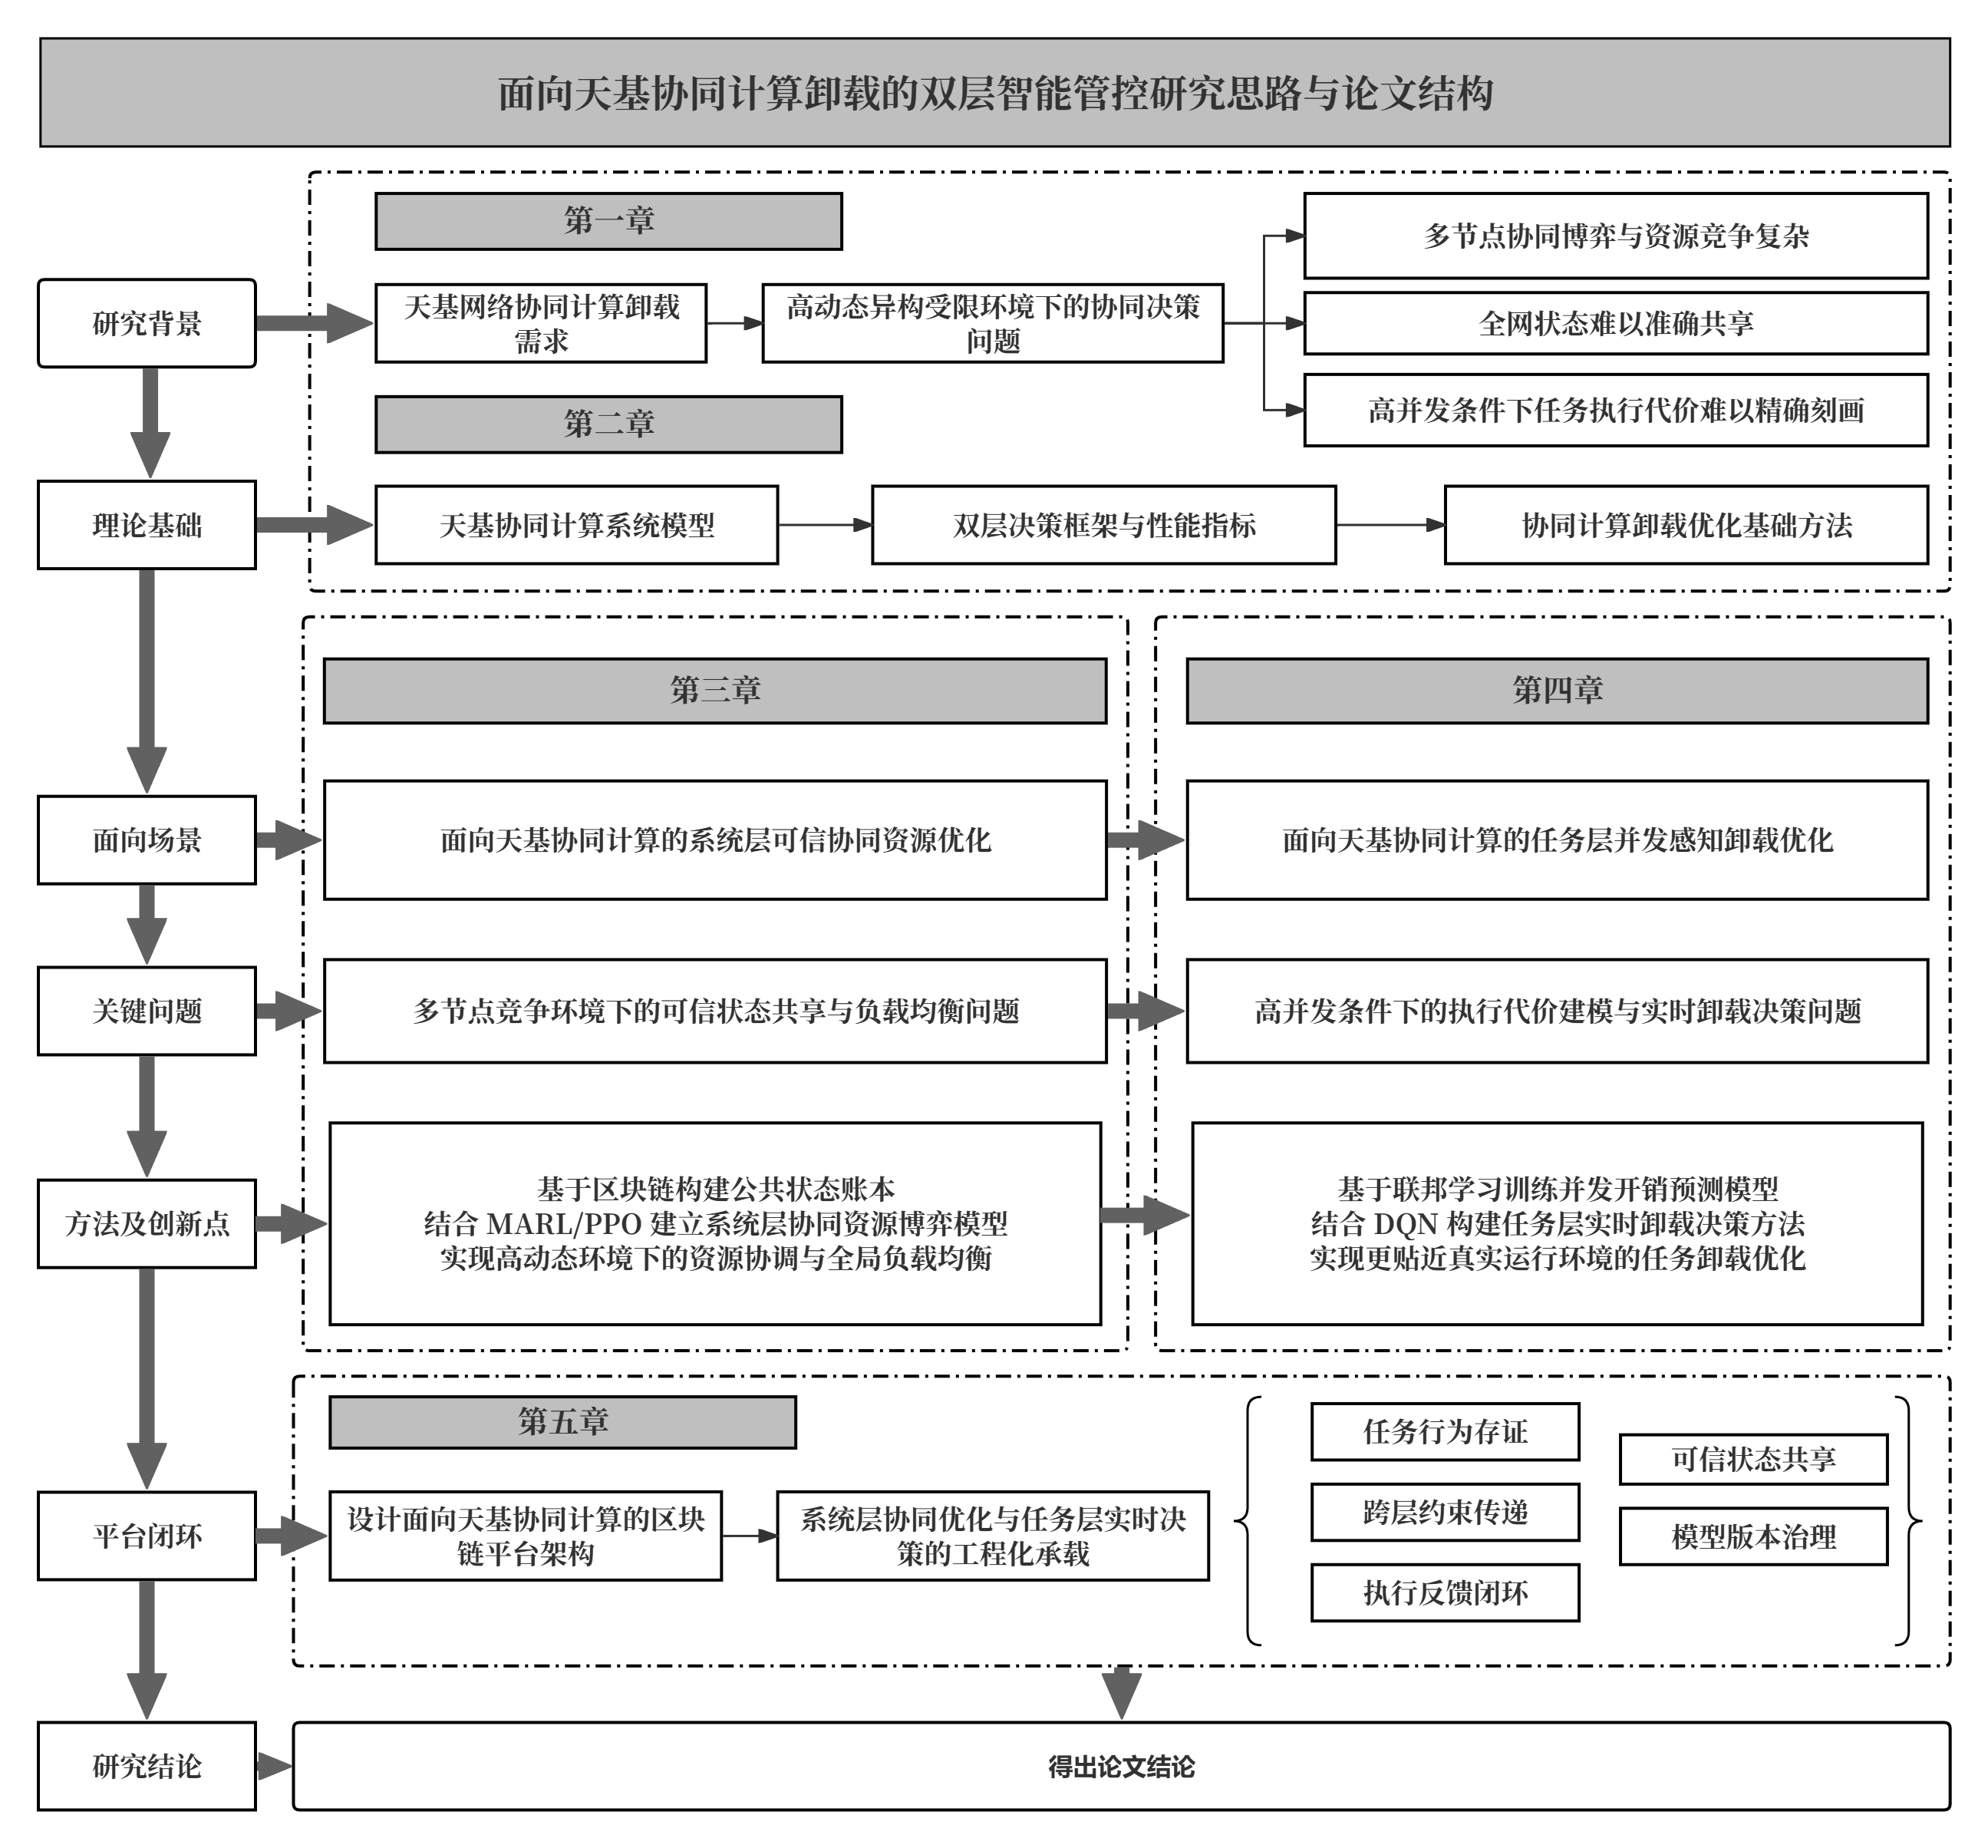
\includegraphics[width=0.85\textwidth]{figures/1-3.png}
  \caption{本论文研究思路及文章结构}
  \label{fig:structure}
\end{figure}

针对本文的研究工作，具体内容和章节安排如下：

第一章为绪论。首先介绍天基网络协同计算卸载的研究背景与意义，分析天基网络由传统转发网络向分布式协同计算平台演进的现实需求，以及在高动态、去中心化环境下面临的状态共享、资源协同、实时决策与平台承载等关键问题。其次，从天基边缘计算与任务卸载、动态环境下智能调度与多智能体协同、区块链协同与隐私保护学习三个方面，对国内外研究现状与发展趋势进行梳理。在此基础上，总结现有研究存在的主要问题与挑战，并给出本文的研究内容与整体结构安排。

第二章主要研究面向天基协同计算卸载的系统模型与理论基础。首先，结合卫星节点异构、链路时变、任务随机到达以及资源受限等特征，建立天基协同计算系统模型，形成对节点、任务、链路和资源约束的统一描述。其次，围绕系统层协同与任务层卸载所涉及的关键问题，梳理可信共享、多智能体协同、联邦学习和深度强化学习等相关理论基础，为后续章节的方法设计提供建模依据和理论支撑。

第三章研究基于区块链与MARL/PPO的系统层可信协同资源博弈方法。针对天基网络中全局状态难以准确获取、多节点之间易出现资源竞争与负载失衡的问题，构建面向系统层协同优化的可信状态共享与多智能体博弈框架。通过将区块链机制引入分布式状态维护过程，实现多节点资源信息的可信记录与共享；在此基础上，将多个卫星节点建模为多智能体，利用PPO策略优化实现系统层的协同资源调度与负载均衡。通过该章研究，为后续任务层卸载决策提供可信状态基础和系统协同环境。

第四章研究基于联邦学习与DQN的任务层并发感知卸载方法。针对传统卸载模型难以准确刻画多任务并发执行代价的问题，构建面向任务层实时决策的并发感知建模与智能卸载方法。首先，结合节点内部任务排队、资源争用和运行扰动等因素，建立更贴近真实运行环境的执行代价建模思路；其次，引入联邦学习机制，在保护各节点本地数据隐私的前提下完成并发代价预测模型训练；进一步结合DQN方法，将任务特征、链上状态和并发代价预测结果映射为具体卸载动作，实现面向动态环境的实时任务卸载优化。

第五章研究面向天基协同计算的区块链平台架构与运行机制。针对现有相关研究中算法设计与系统实现相互割裂的问题，在前述系统模型与双层智能方法基础上，设计能够统一承载可信共享、协同优化、模型治理与任务执行反馈的区块链平台架构。通过构建链上治理与链下计算相结合的运行机制，实现系统层与任务层方法的协同集成，为双层智能方法的工程化部署与可持续运行提供支撑。

第六章对全文工作进行总结，并对后续研究方向进行展望。